\subsubsection{Text comparison function}

We tried to figure out how the text comparison function works. First we just ''translated'' every code line from Javascript into PHP. It was not difficult to rewrite the code, but it took much time and effort to find and fix the errors. We had to debug most of  the code lines. In some cases we found out that it did not work because some issues seem to be the same thing in both languages, but actually if they were written in PHP, they had a different meaning than if they were written in Javascript.

For example we had to check, if a key named \textit{match\_tag} existed in a hash table named \textit{match\_table}. If yes, the value for this key will be added. In the JavaScript version, they used \textit{if (match\_tag in match\_table)}, where it did not matter if \textit{match\_tag} was a key or a value. In PHP version, the equivalent function \textit{if(in\_array(\$match\_tag, \$match\_table))}, was used. We thought it would be the same thing like in Javascript, but the result we received was always an empty array. After several times debugging we realized that it was about an associative array in PHP and this function searched only for the value. We had to check for the key and \textit{if(array\_key\_exists(\$match\_tag, \$match\_table))} had worked finally.

Another example for the diversity of the same issues in different languages was the different meaning of NULL. In Javascript NULL means an object with no initial value, in PHP it means 0, empty or false (3). So there were some places in the code declared with NULL, it should be changed to -1 in PHP (we chose -1, just a different value, sothat it would not return to an empty object, which we did not have in the code) in order to receive the expected result. 
\footnote{http://php.net/manual/en/types.comparisons.php}

After fixing all the errors, we got a nice text comparison function in PHP. The final result is an array of token lists in the form:

\begin{lstlisting}
array{doc_1, start_token_1, doc_2, start_token_2, length} 
\end{lstlisting}

where doc\_X are indices into the documents array, and start\_token\_X are indices into the respective token list of the documents, length is the default length of a phrase. 
\footnote{http://de.vroniplag.wikia.com/wiki/MediaWiki:Fragcolors/code.js}

For example we had two dummy inputs

\begin{figure}[!h]
  \centering
  \fbox{
    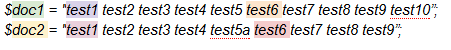
\includegraphics[width=0.97\textwidth]{images/sim_ex_1.png}
  }
  \caption{simtext result}
  \label{fig:simtext _result}
\end{figure}

Here was the matches

\begin{figure}[!h]
  \centering
  \fbox{
    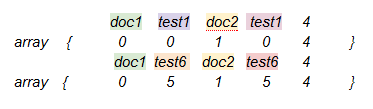
\includegraphics[width=0.97\textwidth]{images/sim_ex_2.png}
  }
  \caption{simtext result}
  \label{fig:simtext_result}
\end{figure}
The result was presented on browser

\begin{figure}[!h]
  \centering
  \fbox{
    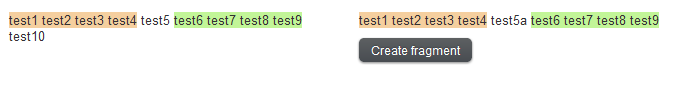
\includegraphics[width=0.97\textwidth]{images/sim_result.png}
  }
  \caption{simtext result}
  \label{fig:report_deckblatt}
\end{figure}